\documentclass[10pt]{acmsiggraph}               % final
%\documentclass[review]{acmsiggraph}      % review
%\documentclass[widereview]{acmsiggraph}  % wide-spaced review
%\documentclass[preprint]{acmsiggraph}    % preprint

%% Uncomment one of the four lines above depending on where your paper is
%% in the conference process. ``review'' and ``widereview'' are for review
%% submission, ``preprint'' is for pre-publication, and ``final'' is for
%% the version to be printed.

%% These two line bring in essential packages: ``mathptmx'' for Type 1 
%% typefaces, and ``graphicx'' for inclusion of EPS figures.

%\usepackage{mathptmx}
\usepackage{graphicx}

%% use this for zero \parindent and non-zero \parskip, intelligently.

\usepackage{parskip}

\usepackage{amsmath}

% Define some useful commands
\newcommand{\bm}[1]{\boldsymbol{#1}}

%% need to document this!
\acmformat{print}


\title{Conditional Random Fields for the Classification of Digital Logic Circuits\\
\small{July 2006}}

\author{Jason Fennell\\ Harvey Mudd College \\ jfennell@hmc.edu
\and Max Pflueger\\ Harvey Mudd College \\ mpflueger@hmc.edu }

%% Keywords that describe your work.
\keywords{}

%%%%%% START OF THE PAPER %%%%%%
\begin{document}

\maketitle

\begin{abstract}
Sketches are an important and natural means of communication that historically have been of little use as a way of interacting with computers.  A sketch recognition interface to computers with the capability to recognize the meaning of sketches would increase both the ease of use and usefulness of computers for design.  We addressed stroke-level recognition by constructing a Conditional Random Field that uses the context in which strokes are drawn to improve recognition.  We have successfully used this tool to distinguish between wires and gates in sketches of digital logic circuits, a domain that is more complex than domains considered in previous work.
\end{abstract}

\section{Introduction}

Sketches are a natural medium of communication used regularly in engineering, computer science, and many other fields.  While they are excellent tools for communicating with other humans, they are limited by the inability of computers to recognize and analyze them. If sketches were a natural way of communicating with computers, it would improve the ease of use of computers for desgin and other processes.

Our research focuses on the problem of recognizing a freely drawn sketch with the eventual goal of developing a natural computer interface.  This problem presents us with two main challenges. First we must cope with the variability and sloppiness inherent in sketches.  Second, it is difficult to determine exactly how to partition the strokes of a sketch (strokes are considered to be a continuous motion of the pen across the tablet surface) into the objects the user intends to represent. This process is called segmenting.  If one has access to segmentation data on a sketch, sketch recognition becomes a much easier problem, since the number of individual elements to be recognized shrinks and there is more information contained in each of these elements. 

Our overarching goal is to create a toolchain that can take as input a sketch of a digital circuit and output a fully recognized version of that circuit in a design program.  We restrict ourselves to recognizing digital circuits to limit the complexity of our problem.  Additionally, to give the user a natural interface we do not contstrain the them in any way during the sketching process.  Adding interface requirements, such as having users indicate segmentation of their sketch for us, would make our task significantly easier.  However, such restrictions have a negative effect on the

This paper focuses on the problem of recognizing individual strokes in a sketch, a low-level step in our toolchain. The goal of our stroke-level recognition is to inform a segmentation tool and improve its accuracy. Before this recognition is performed the sketch is fragmented into lines and arc-segments to give us more strokes to train on, and simpler strokes to recognize. For more information on the fragmentation, see the report by Aaron Wolin \cite{wolin:fragmenter}.  After the stroke-level recognition has finished another program uses the recognized strokes to segment our drawing into logical parts by grouping sets of strokes that make up gates or wires together.  This segmenter goes back and forth with an object-level recognizer that attempts to recognize the objects the segmenter found.  For more information on segmentation and recognition, see the report by Devin Smith \cite{smith:segmentation}.  Once this final recognition step is complete, the circuit undergoes analysis and is passed to a design program, fully understood by the computer.

The sparsity of information contained within individual strokes presents the major challenge for stroke based recogntion.  The stroke making up the back of an AND gate can look exactly the same as a small piece of wire.  However, a stroke's context can provide significantly more information about what a stroke means.  We use context to mean a stroke's relationship to the strokes near it in time and space, or to all of the other strokes in the input.  Context is the key to our solution of the stroke-level recognition problem.  A straight line that is connected on both ends to an arc can be recognized as the back of an AND gate, whereas another straight line that looks exactly the same is recognized as a wire when it has two different straight lines touching either end.  

It is with the importance of context in mind that we have constructed a Conditional Random Field, or CRF, to perform stroke-level recognition. A CRF uses the context and stroke data to classify the stroke. The CRF consists of two parts: a graph that encodes the probabilistic dependencies between the elements of the CRF input (strokes in our case), and an associated set of potential functions that measure the compatibility between labels and strokes over cliques in the graph.  The CRF incorporates contextual information through the potential functions, which measure compatability of individual labels and strokes as well as compatibility between groups of mutually dependent labels and strokes.  For instance, a potential function could quantify how compatible neighboring strokes are if the first is labeled wire and the second is labeled gate.  Once the graph and potentials are constructed, the CRF can be given to an inference algorithm that calculates the probability of each possible label on every input.  These probabilities are used to select the most likely set of labels for the input.  

Our goal for the CRF is to correctly classify strokes in digital logic circuits to provide a major piece of a sketch recognition toolchain.  We have extended two-label classification into the domain of digital circuits---which is a more complex domain than considered in previous research---with a high level of accuracy.  We have also made headway with multi-label classification in the same domain.  We begin with a closer look at CRF's in general, then discuss our implementation and results.

\section{Background}

Szummer and Qi offer an excellent explanation of Conditional Random Fields in their paper ``Contextual Recognition of Hand-drawn Diagrams with Conditional Random Fields'' \cite{szummer:CRFrecog}. We summarize their exposition below.

A Conditional Random Field is an undirected graphical model that seeks
to find the joint probability distribution $P(\bm{y} | \bm{x} )$ where
$\bm{x}$ is a set of input data and $\bm{y}$ is a set of labels for
that input data.  The actual CRF consists of a graph $G = (V,E)$ and
an associated set of potential functions.  Each node in $V$
corresponds to an element of the input $\bm{x}$, and each edge in $E$
quantifies a probabilistic dependence between nodes.  $G$ thus obeys
the Markov property, which means that the probability that a node has
a label is dependent only on neighbors.  Formally, $P(y_i | \bm{x},
\bm{y}_{V-i}) = P(y_i | \bm{x}, \bm{y}_{{\cal N}_i})$, where
$\bm{y}_{V-i}$ is all of the nodes other than $i$ in the graph, and
$\bm{y}_{{\cal N}_i}$ is the neighborhood of $i$
~\cite{szummer:CRFrecog}.

There are two types of potential functions: site potentials that are
associated with each node, and interaction potentials that are
associated with each pair of nodes.  In theory, potentials could exist
over cliques larger than 2, but this makes the CRF prohibitively
complex.  The intuitive understanding of a site potential function is
that it measures the compatibility between a label and a node.
Similarly, an interaction potential measures the compatability between
a pair of labels and a pair of adjacent nodes.  Both types of
potentials measure compatability by linearly combining parameters with
a set of feature functions and passing the result through a
non-linearity.

A feature function takes as input some subset of the input data and
returns a numerical representation of a charactaristic of that
data. As with potentials, feature functions come in two varieties,
site features and interaction features. Site features are functions of
a single node, and interaction features are a function of an adjacent
pair of nodes.  An important property of CRF feature functions is that
while they are functions measuring compatibility between up to two
labels and nodes, they have access to all of the input data $\bm{x}$,
not just the data for the nodes in question.

Parameters are associated with every feature function, and quantify
how important each feature is to the classification of a node or pair
of nodes with a certain label.  If $l$ is the number of labels the CRF
has to decide between, each site feature has $l$ parameters associated
with it and each interaction feature has $l^2$ parameters associated
with it, one for every label or pair of labels that can be applied.
Putting this all together, potential functions take the form:

\begin{align*}
\textrm{Site:} &\qquad \Phi(y_i, \bm{x}; \bm{\theta}) = e^{\bm{\theta}(y_i) \cdot \bm{g}_i(\bm{x})} \\
\textrm{Interaction:}& \qquad \Omega(y_i, y_j, \bm{x}; \bm{\theta}) = e^{\bm{\theta}(y_i,y_j) \cdot \bm{f}_{i j}(\bm{x})}
\end{align*}

Where $\bm{\theta} = [ \bm{w \; v} ]$ and $\bm{w}$ is the set of
parameters for site features and $\bm{v}$ is the set of parameters for
interaction features.  Also, $\bm{g}_i$ is the vector of site features
for node $i$ and $\bm{f}_{i j}$ is the vector of interaction features
between nodes $i$ and $j$.  The probability distribution
$P(\bm{y}|\bm{x},\bm{\theta})$ that we are interested in can be
factored into a product of these potential functions using the graph
$G$.  This gives the following probability distribution that the CRF
models:

\begin{align*}
P(\bm{y}|\bm{x},\bm{\theta}) = {1 \over Z(\bm{\theta})} \prod_{i \in V} \Phi_i (y_i,\bm{x};\bm{\theta}) \prod_{(i,j) \in E} \Omega_{i,j} (y_i,y_j,\bm{x};\bm{\theta})\\
Z(\bm{\theta}) = \sum_{\bm{y}} \left( \prod_{i\in V} \Phi_i (y_i,\bm{x};\bm{\theta}) \prod_{(i,j) \in E} \Omega_{i,j} (y_i,y_j,\bm{x};\bm{\theta})\right)
\end{align*}

The probability above can be calculated using an inference algorithm which will calculate $P(y_{i}|\bm{x},\bm{\theta})$ which can then be used to calculate $P(\bm{y}|\bm{x},\bm{\theta})$.

\subsection{Training}

Training the CRF consists of finding the set of parameters (a point in parameter-space) that maximizes the log of the likelihood $P(\bm{y}|\bm{x},\bm{\theta})$, which takes the form

\[
	\mbox{$\mathcal L$} = \sum_{i \in V} \bm{w}(y_i) \cdot \bm{g}_i (\bm{x}) + 
	\sum_{(i, j) \in E}	\bm{v}(y_i, y_j) \cdot \bm{f}_{i j} (\bm{x}) - 
	\mathrm{log}Z(\bm{\theta}) -
	\frac{||\bm{\theta}||^2}{2\sigma^2}.
\]

After initializing $\bm{\theta}$ with random Gaussian priors, we train using Nonlinear Conjugate Gradient Descent by following the gradient of $\cal L$ toward the critical
point of our surface.  Other work, such as \cite{szummer:CRFrecog} has also had success with the quasi-Newtonian BFGS method.  The gradient of $\cal L$ takes two different
forms depending on whether differentiation is done with respect to site or interaction parameters. 

\[
	\frac{\mathrm{\partial}\mbox{$\mathcal L$}}{\mathrm{\partial}\bm{w}(y_i)} = 
	\sum_{i \in V} \bm{g}_i (\bm{x}) - 
	E \left(\sum_{i \in V} \bm{g}_i (\bm{x})\right)
	 - \frac{\bm{w}(y_i)}{\sigma^2}
\]

\[
	\frac{\mathrm{\partial}\mbox{$\mathcal L$}}{\mathrm{\partial}\bm{v}(y_i,y_j)} = 
		\sum_{(i, j) \in E} \bm{f}_{i j} (\bm{x}) - 
		E\left(\sum_{(i, j) \in E} \bm{f}_{i j} (\bm{x})\right)
		 - \frac{\bm{v}(y_i,y_j)}{\sigma^2}
\]

Where $E$ denotes the expected value of a function with respect to the current model distribution $P(\bm{y}|\bm{x},\bm{\theta})$.  Note that this is simply shorthand, as $E \left(\sum_{i \in V} \bm{g}_i (\bm{x})\right) = \sum_{\bm{y}} \left(\sum_{i \in V} \bm{g}_i (\bm{x}) P(\bm{y}|\bm{x},\bm{\theta})\right)$.  There is a similar formula for interaction features.

\subsection{Similar Problems}

Earlier research has used CRFs and variants on CRFs to classify hand drawn diagrams, however, we are not aware of anyone who has used it for such a complex set of possible labels.  Previous research by Szummer and others has shown great success in using CRF's to classify strokes in organizational charts involving connectors (lines) and containers (simple geometric shapes, usually rectangles) \cite{szummer:CRFrecog}, \cite{szummer:HRF}, \cite{cowansSzummer}. These papers, especially \cite{szummer:CRFrecog}, form the jumping off point where our own project began.  

For a more in depth treatment of CRF's, refer to \cite{wallach:CRFintro}, \cite{sutton:CRFintro}

\section{Approach}

Our purpose in implementing a CRF is to correctly label the individual strokes in a digital logic circuit sketch
to allow for further recognition of the sketch.  With this in mind we begin our discussion of the specific
implementation of CRF that we have created, and the important aspects of the design.

\subsection{Fragmenter}
Before the CRF begins to work on our data, the strokes have to be fragmented.  The purpose of the fragmenter is to divide strokes up into lines and arcs. Additionally, and perhaps more importantly, in the occasional case when one stroke will be used to draw two distinct elements of the diagram, it is the job of the fragmenter to divide that stroke between those two elements so they can be properly recognized by the CRF. The quality of the results obtained from our CRF is highly dependent on the quality of the fragmentation of the data. Further discussion of this is in the results section. 

\subsection{General CRF}
Our implementation of a CRF allows for a completely general graph to encode the probabilistic dependencies of the input.  The graph is constructed by making a node for every stroke in the input sketch, and placing edges between nodes that differ by less than a temporal or spacial theshold.  These thresholds are currently rather arbitrary (about 2 seconds and 1 centimeter respectively).  Hopefully later research will be able to fully optimize these values.

%This paragraph might be cut for publication
There are a number of simplifying assumptions that can be made about the structure of a CRF's graph to lessen computational complexity.  CRF implementations often assume that the graph will take the form of a linear chain, or a two-dimensional lattice.  However, neither of these limited models can accuratly represent the interactions of a hand-drawn sketch, and hence these assumptions are unacceptable for our application.

\subsection{Multi-Label}
We designed our CRF to handle an arbitrary number of labels. A multi-label CRF is very similar to a two label CRF mathematically, but computationally there are some notable differences. First, the number of parameters grows as $O(l^2)$ where $l$ is the number of possible labels. The number of parameters grows this way because the interaction features on an edge must be calculated for every possible label combination, of which there are $l^2$. 

An individual CRF is represented by its parameter space. The parameter space comes in two parts, the site parameters and the interaction parameters. If the number of labels is $l$ and the number of site feature functions is $s$, the number of site parameters  is $l\times s$ because there is a parameter for each site feature function associated with each label.  If the number of interaction feature functions is $i$, then the number of interaction parameters is $l^2\times i$ because there is a parameter for each interaction feature combined with a pair of labels.

For a system with $m$ possible states there are $m-1$ decision boundaries, therefore there are $l-1$ decision boundaries on nodes for each feature function and $l^2-1$ decision boundaries on edges for each feature function. The number of parameters must match the number of decision boundaries, otherwise you have redundant parameters that could lead to wandering parameter values. To avoid this, we zero out the set of site parameters for the first label (label 0) and the set of interaction parameters for labels (0,0). 

\subsection{Feature functions}
One of the most important aspects of the performance of a CRF is the selection and design of feature functions.  As mentioned previously, feature functions can either be site features of nodes or interaction features of a pair of adjacent nodes.  A typical site feature may compute something such as the length of a stroke, or a stroke's degree of curvature. A typical interaction feature may compute something such as how close the ends of two strokes are to each other or whether or not two strokes cross each other.

Unfortunately, to get good results it is not as simple as just outputting values such as length or curvature. The CRF behaves in a linear fashion on the feature functions, but the relationships between these functions and the useful data about the sketch is almost always non-linear. For example, consider a feature function that measures how much a stroke curves across its length.  If a particular stroke does a half-turn, then it may be the front of an AND gate. However, if that stroke turns more it is certainly not more of an AND gate than before, and a full turn is not twice as much AND gate as a half-turn. In order to deal with this we broke up features, such as curvature, into groups of features, each associated with a certain region of the output of the function in question. For example, we might have one function that indicates a very small curvature, another that indicates a medium curvature, and yet another that indicates a large curvature. Breaking up scalar valued feature functions in this way allows us to have more complex recognition behavior across the range of the function. The decisions about where to break up the scalar valued features were made based upon preliminary observations of the data. The output of these new feature functions is a value in the range of 1 to -1 to represent true or false. Most of the time this value is very close to 1 or -1, but for input near the boundary of the function we used a smooth transition between 1 and -1.

If scalar valued feature functions are to be included, they must be normalized so they do not exceed a reasonable range, in our case something like a maximum absolute value of 10 to 15. By breaking up the scalar valued feature functions we get the added benefit of fixing the range of our feature functions.  Later in the algorithm we compute the exponential of the feature functions. This means that, if the values from feature functions become too large, the exponential will very quickly exceed the range of a double, causing the program to fail. 

\subsection{Inference}
Exact algorithms for inference on graphs with loops are intractable for even very small graphs.  To perform inference on our CRF we used the loopy belief propagation algorithm, as implemented by Kevin Murphy in his CRF Toolbox \cite{murphy:CRF}. Loopy BP is an approximate inference algorithm adapted for graphs with loops from the standard belief propagation algorithm. It is not guaranteed to converge, and occasionally causes problems during execution. 

\subsection{Training}
In this section we outline the salient details of the training methods we used on our CRF.  First we mention our use of the Conjugate Gradient method to do training.  We then explain one of the problems that we have had in training and our implementation of ShakeIt! to fix that problem. Next is an explanation of the regularization of our gradient and log-liklihood functions, and finally is an explanation of the method of preconditioning which we used to greatly increase how well our training worked.

By adjusting the parameters $\bm{\theta}$, training seeks to minimize $-\cal L$ the negative log-likelihood of our CRF, so that the set of correct labels for the training dataset are the most likely.  We used Non-linear Conjugate Gradient Descent for training our CRF.  This is an extension of the simple gradient descent algorithm, so the basic concept behind the algorithm is to use the gradient of a function to step toward a critical point of the surface in question.  For more information about Non-linear Conjugate Gradient Descent, see ``An Introduction to the Conjugate Gradient Method Without the Agonizing Pain'' by Jonathan Shewchuk \cite{shewchuk:ConjGrad}.

Note that the gradient and log-liklihood functions, and thus training, need $\log Z(\bm{\theta})$ to be calculated.  This value is in turn found as part of the Loopy BP calculation.  Occasionally in the course of training a negative or otherwise obviously wrong value of the $\mathcal L$ function is returned. We suspect that these values are due to Loopy BP not converging and returning an incorrect value for the $\log Z(\bm{\theta})$ term. However, regardless of the source of these errors, uncorrected they will cause the training to fail. Hence, we added a piece of code that looked for such erroneous values, and fixed them by slightly randomizing the current set of parameters and recalculating until an acceptable value was arrived upon. We call this the ShakeIt! code.

Adding regularization factors to our log-likelihood and gradient functions improved our training significantly.  This is the $\frac{||\bm{\theta}||^2}{2\sigma^2}$ term in $\cal L$, the $\frac{\bm{w}(y_i)}{\sigma^2}$ term in $\frac{\mathrm{\partial}\mbox{$\mathcal L$}}{\mathrm{\partial}\bm{w}(y_i)}$, and the $\frac{\bm{v}(y_i,y_j)}{\sigma^2}$ term in $\frac{\mathrm{\partial}\mbox{$\mathcal L$}}{\mathrm{\partial}\bm{v}(y_i,y_j)}$.  These terms serves two purposes:  without it the values of the parameters have the tendency to explode and cause numerical overflow errors, and it also prevents the training algorithm from overfitting.  We have set $\sigma^2$ to a hard value for our implementation, but others recommend more complex methods for finding its value \cite{szummer:HRF}.

Because of the difficulty in getting the CRF parameters to converge to
a good value in a single run, we use preconditioning by training first
on smaller sets of data to get parameters that are close to the
optimal parameters.  We will also sometimes run training on smaller
datasets between training runs on full datasets to perturb the
parameters slightly in the hope that the next full training set will
converge better.  The imperfect nature of nonlinear conjugate gradient
descent and the possibility that Loopy BP will not converge mean that
the CRF parameters do not always converge all the way, in fact,
usually they stop well before their optimal point. The process running
the same set of CRF parameters through successive rounds of training
on differing data sets has the effect of defeating these imperfections
by starting closer to the optimal point at the beginning of each round
of training.

\section{Results and Discussion}

To obtain data on which to run CRF training and classification, we
surveyed other computer science researchers working nearby us.
Generally our subjects had a passing familiarity with digital circuits
and little to no experience with tablet computers.  We asked them to
draw copies of the circuits in Figure \ref{example1} and Figure
\ref{example2}, then to design a circuit of their own choosing using
AND, OR, NOT, and NAND gates. The final circuit was not required to
have any formal meaning other than being correct (only one input for a
NOT gate, for example).  Subjects were told that they would not be
judged on performance.

We collected a total of 51 circuit diagrams.  We trained on a chosen
subset of the circuit sketches, generally using 17 samples for full
training and 4 or fewer samples for conditioning.  We classified the
remaining diagrams.  We also excluded the third sketch of one of our
users because it is apparent that they were trying to draw a smiley
face with circuit components rather than trying to draw an actual
circuit.

\begin{figure}[h]
\centering
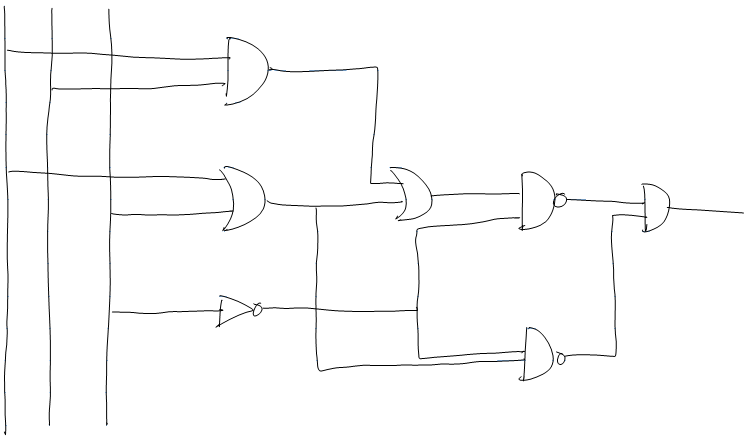
\includegraphics[width=1.8in]{example1.png}
\caption{First example subjects were asked to draw.}
\label{example1}
\end{figure}

\begin{figure}[h]
\centering
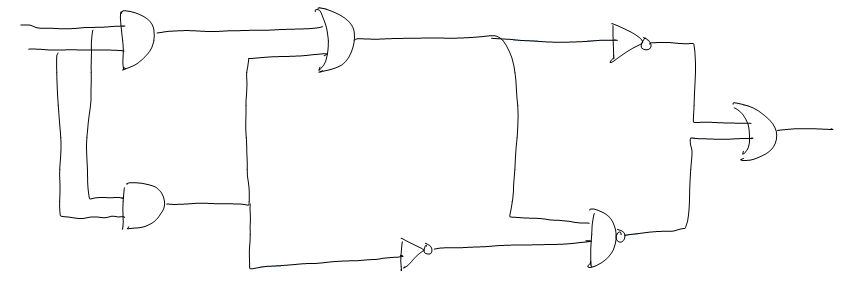
\includegraphics[width=1.8in]{example2.png}
\caption{Second example subjects were asked to draw.}
\label{example2}
\end{figure}

\subsection{Fragmenter}
The recognition performance of the CRF is highly dependent on the how the sketch is fragmented. An underfragmented sketch, or a sketch that is not fragmented at key points is difficult for the CRF to recognize because the strokes do not come in predictable shapes, or one stroke may be used in two different elements.  Going the other direction, an overfragmented sketch is difficult to recognize because the strokes may be decimated to the point of not being individually significant, giving the CRF very little evidence per node.  Fragmenting is a difficult problem in and of itself, and we will not discuss the precise details of that project here.  The fragmenter is explored in depth in a paper by Aaron Wolin \cite{wolin:fragmenter}.

\subsection{Two label classification}
Two-label classification attempted to label the strokes in a sketch as
either Wire or Gate.  We ran four training runs on our data for
two-label classification, all four of which followed the training
procedure outlined at the start of this section.

The first run trained on all seventeen of the sketches of Figure
\ref{example1}, and conditioned on four sketches of Figure
\ref{example2}.  The second run used the same datasets as the first,
but was run on modified $\sigma$ values.  For this run our parameters
were initialized randomly from a normal distribution with a standard
deviation of ${1 \over 3}$ instead of 1.  We also changed the
$\sigma^2$ in our regularization term in $\cal L$ and gradient so that
$\sigma = {1 \over 3}$.  Our third training run used the original
$\sigma$ values from the first run as well as seventeen training
examples chosen randomly from the sketches of Figures \ref{example1}
and \ref{example2}, and four conditioning examples chosen similarly.
Finally, our fourth run used the original $\sigma$ values.  Seventeen
training examples were chosen randomly from all of the sketch data,
and four conditioning examples were chosen similarly.  Running
classification as outlined at the start of the section gave us the
results seen in Table \ref{results}.

\begin{table}[h]
\begin{center}
	\begin{tabular}{|c|c|}
		\hline
		Train on: & Mean Recognition Rate\\
		\hline
		Fig \ref{example1} & $93 \pm 2$\%\\
		\hline
		Fig \ref{example1}, $\sigma={1 \over 3}$ & $93 \pm 2$\%\\
		\hline
		Rand. subset of Fig \ref{example1} \& \ref{example2} & $92 \pm 1$\%\\
		\hline
		Rand. subset all sketches & $96 \pm 1$\%\\
		\hline
	\end{tabular}
\end{center}
\caption{Two-label classification results}
\label{results}
\end{table}

There was no statistically significant change in recognition rates
when we changed $\sigma$, or opened up the training set to both the
first and second sketches.  The only statistically significant change
was the increase in performance from training on a subset of all of
our data This seems to indicate that training on a representative and
broad subset of data is necessary for good recognition.

One qualitiative observation from classification is that interaction
features that detected grouping of strokes seemed to have both the
largest parameter values when two strokes were given the same label
and the largest absolute parameter values we saw. An example of such a
feature is one that detectes if a two strokes were originally part of
the same stroke (before fragmentation).  The largest parameter being
given to strokes with the same label indicates that these features
tend to create clusters of nearby strokes all with the same label.
The fact that these parameters were the largest in absolute terms
indicates that this type of clustering of nearby, like-labeled strokes
is one of the strongest behavior of the CRF.  This behavior is most
obvious empirically when there is a misclassified wire in a sketch.
When this happens, all of the strokes that made up the original wire
(that was drawn in one stroke) are all misclassified.

One interaction feature that exhibited just the opposite of this
grouping behavior is the T-junction checking function.  This function
had large absolute support for the cross of the junction to be a Gate
and the stem to be a Wire.  This feature seems to have played a large
role in delimiting between like-labeled groups of strokes, breaking
them up into their proper segments.

\subsection{5-label classification}

In addition to simple binary classification we have extended the CRF
to do classification between an arbitrary number of labels. Five-label
classification tries to label strokes as Wire, AND, OR, NOT, or NAND.
There was only one successful training run for five-label
classification.  The training process for five-label classification
has only minor modifications from the training on two labels.  We
added a conditioning step on three sketches before the first training
run, and the conditioning between training runs only used three
sketches, one of which was the same as used in the first conditioning
step.

Classification on the remaining sketches yielded a mean recognition rate of $39 \pm 2$\%.  While the recognition rate is low, it is still well above random chance.  Also, quite frequently there were gates in the survey input that could not be recognized accurately by humans because of the sloppiness of the drawing.  

\subsection{Discussion}

What sorts of errors does it make? What does it recognize reliably.

\section{Related Work}

Conditional random fields were originally introduced by John Lafferty et. al. in the the paper ``Conditional Random Fields: Probabilistic Models for Segmenting and Labeling Sequence Data'' \cite{lafferty01conditional}.	
A major jumping off point for our work has been the paper by Szummer and Qi, ``Contextual Recognition of Hand-drawn Diagrams with Conditional Random Fields'' \cite{szummer:CRFrecog}. The paper provides a detailed approach and much of the theory necessary to apply a general, dynamically generated CRF to sketch recognition.	
A similar model to conditional random fields known as hidden random fields is used by Szummer in his paper ``Learning Diagram Parts with Hidden Random Fields'' \cite{szummer:HRF}. This approach is derived from to conditional random fields, and does not seem to show a significant gain in performance over CRFs.
In our approach we chose to do only labeling with our CRF, and segment the strokes later. However, not everyone has taken this approach. Cowans and Szummer have created a graphical model that simultaneously does partitioning and labeling \cite{cowansSzummer}. Although their approach shows significant promise in accuracy, the computational cost is very high. 

\section{Future Work}

There are many different paths that future research on this subject can take, largely with the hope
of improving the overall recognition accuracy of the CRF.  The first and simplest way
in which classification could be improved is by doing a study of the behavior of our current CRF and
its feature functions, and tweaking the large number of arbitrary values in the code.  These arbitrary values
primarily crop up as thresholds in our binary feature functions that find if a scalar valued feature function falls in a certain
region.  We would hope to optimize the borders of these regions.  Also, the
algorithm that creates edges in the CRF's graph uses hard time and space threshold values, which we would also
like to study and optimize.

A major aid to any future work with CRFs would be a solid theory of how different types of feature functions effect recognition.
We propose a study to examine how performance in training and classification changes as the feature functions
are altered over a fixed set of data.  In the course of this study, there are a number of areas that should be addressed.

\begin{itemize}
\item The optimal return values for binary features.  Should they return 1 on a positive result and 0 on a negative result, or 1 on a positive result and -1 on a negative result. A value of 1 would always represent the feature being true, but it is unclear what the value should be when the feature is false.  A value of zero would mean that an untrue feature would have no effect on the CRF, whereas, -1 would have the exact opposite of true effect on the results. The decision for us was an easy one, since features that regularly return 0 lead to parameter explosion errors in our code. However, if this problem were fixed, it would be useful to know what the optimal false return value is. Also, should there be some combination of these two schemes based on the type of feature function?  Should binary features instead replace their two return values with a transfer function between 1/0 (or 1/-1) that indicates the strength of the feature toward one end or the other, or does this simply turn a binary feature into a bounded scalar feature?

\item Creation of region based binary features from scalar features.  An as yet unsolved problem for us is the decision of where to break up the scalar valued feature functions. The easy solution would be to simply create a very large number of regions, but this would be computationally expensive, and would make training more difficult as there would be a larger number of parameters to properly fit. Our feature functions were broken up with preliminary observations about where logical regions would exist. A method of verifying the usefulness of these regions would be desirable.

\item Normalization of feature functions.  Without small valued features, numerical overflow errors cause the CRF to fail.  It seems like normalization is necessary for the CRF to work. However, is there a way to get the CRF to work without individually normalizing the feature functions, and how do different normalization schema effect classification? Also, what about region-based binary features versus scalar valued features? Do binary features that decide if a scalar valued function is within a given region or not improve upon simple scalar valued feature functions for classification?

\item Symmetry of interaction features.  Are interaction features between nodes required to be symmetric?  Is it enough to have asymmetric feature functions
that come in symmetric pairs / groups?  For instance, a T-Junction function that detects if the first stroke passed to it is the T and the other stroke is the stem is not symmetric.  However, another T-Junction function that detects if the first stroke is the stem and the second is the T would pair with the first function to create a symmetry.  Is this sort of pairing even necessary or can we have totally asymmetric feature functions with no problem?s

\item Combination feature functions.  How does it affect classification to combine multiple active (also being used by the CRF)
features together in some way in another feature.  Will this
allow for more flexible classification (hoping that this would allow two individual features that have a negative effect on a given label to show a positive
effect on the label if they were both negative and that meant some positive effect).
\end{itemize}

The CRF has not done well on higher than two label classifcation.  Improving performance in this area with new feature functions and different training methods should be a priority.

Currently our CRF is needs to be completely retrained if teh feature functions are changed.  We would like to examine the possiblity of chaning the format that we use to store trained CRFs to be tolerant of changes in the feature functions.  XML is a possibility, but other formats could work as well.  This would allow the program to only have to generate random parameters for new feature functions when they are added, instead of losing all the progress of previous training sessions.

There are a number of issues with loopyBP that need to be ironed out.  If it fails to converge, or has any other problems, it causes the CRF to fail.  Also, it is implemented in Matlab and slows down our program.  Reimplementation of loopyBP in C\#, with careful though about how to handle its errors, is necessary for a fast and robust CRF.

%When our CRF fails it is often due to something we called parameter explosion.  This is an error that occurs during training (we don't really have errors during classification), where the training algorithm takes a step along what is nominally the gradient of $\cal L$, and then the CRF falls apart because all of its potential functions have overflow errors and have Positive Infinity for values.  This overflow happens because somehow a bunch of the CRF parameters were inflated to very large values by the first step along the gradient.  These sort of overflow errors have been the bane of our existence, as we have a lot of exponential functions in the code, and when the exponent is anything but small we run into overflow very quickly.  We think that this is why the regularization helped our CRF performance so much.  We however do not know why these parameter explosions occur, though we do know that they cause all the exponential functions to overflow out of doubles when they do occur.  This is something to watch for and hopefully fix in the future.

Finally, there are a few other long term possibilities for improving CRF performance.  Adding the ability 
for there to be a different set (and number) of feature functions associated with each label would be nasty to code,
but has a good chance of improving classification.
Adding interaction features dealing with cliques bigger than size two is more a matter of curiosity than anything, and probably would be very painful to implement.
Also, the CRF should be tried on other sketch domains.

\section{Conclusion}

All that again, but really fast.  Not exactly sure what to say.

\section*{Acknowledgments}
Thanks to all the E85er's and all of the summer 2006 CS researchers on 2nd floor Sprauge
for providing us data.  We also thank Martin Szummer for guiding us through some aspects of
CRF implementation.

\bibliographystyle{acmsiggraph}
%\nocite{*}
\bibliography{crf}
\end{document}

% HERE IS HOW TO INSERT A FIGURE
%\begin{figure}[h]
%\centering
%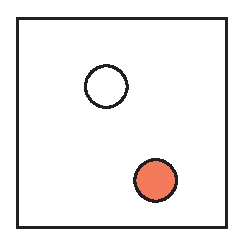
\includegraphics[width=1.5in]{sample.eps}
%\caption{Sample illustration.}
%\end{figure}
